\documentclass[11pt]{standalone}
\usepackage{amssymb}
\usepackage{amsmath}
\usepackage[no-math]{fontspec}
\usepackage{unicode-math}
\usepackage{libertinus}
\usepackage{pgf,xcolor}
\usepackage{tikz}
\usetikzlibrary{arrows.meta, backgrounds}
\usepackage{pgfplots}
\pgfplotsset{compat=newest}

\definecolor{my_darkgray}{HTML}{484949}
\definecolor{my_lightgray}{HTML}{F3F4F4}
\definecolor{my_darkblue}{HTML}{005A94}
\definecolor{my_lightblue}{HTML}{CCDEE9}
\definecolor{my_yellow}{HTML}{FFEC7F}
\definecolor{my_red}{HTML}{E60000}
\definecolor{my_orange}{HTML}{E87846}

\begin{document}
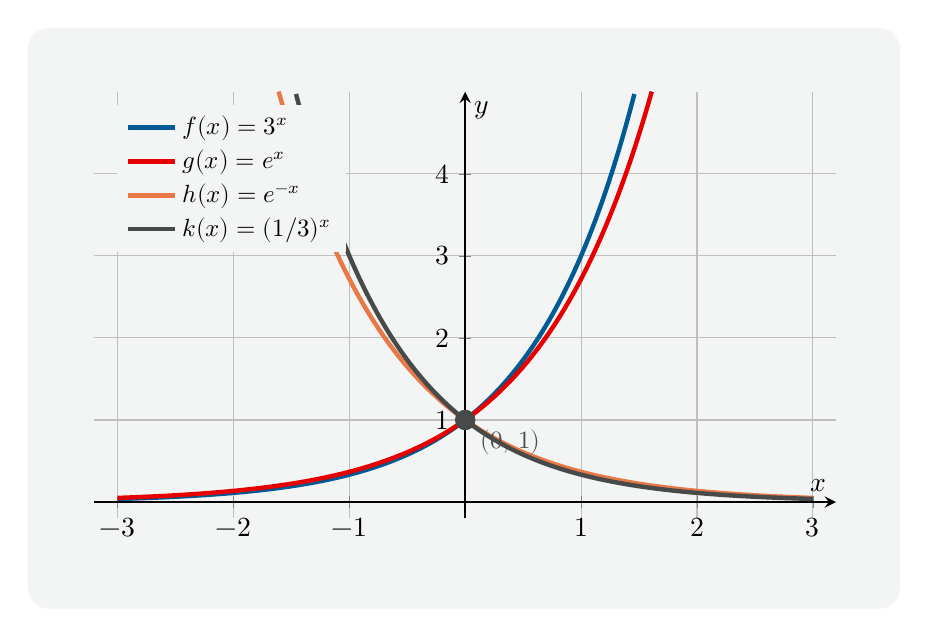
\begin{tikzpicture}[
    show background rectangle,
    background rectangle/.style={fill=my_lightgray, rounded corners=8pt},
    inner frame sep=0.8cm
]
\begin{axis}[
    axis lines=center,
    xlabel={$x$},
    ylabel={$y$},
    height=7cm, width=11cm,
    xmin=-3.2, xmax=3.2,
    ymin=-0.2, ymax=5.0,
    xtick={-3,-2,-1,0,1,2,3},
    ytick={1,2,3,4},
    grid=both,
    axis line style={thick},
    restrict y to domain=-0.5:5.5,
    legend style={
        font=\small,
        at={(0.03, 0.97)},
        anchor=north west,
        draw=none,
        fill=my_lightgray,
    },
    legend cell align=left,
    clip=true,
]

% Four exponential functions: two increasing (a>1), two decreasing (0<a<1).
% All four curves pass through the common point (0,1).

% a = 3: fastest increase (darkblue = primary)
\addplot[draw=my_darkblue, samples=300, ultra thick, domain=-3:1.46]
    {3^x};
\addlegendentry{$f(x)=3^x$}

% a = e ≈ 2.718: natural base (red = secondary)
\addplot[draw=my_red, samples=300, ultra thick, domain=-3:1.61]
    {exp(x)};
\addlegendentry{$g(x)=e^x$}

% a = 1/e ≈ 0.368: natural base, decreasing (orange = tertiary)
\addplot[draw=my_orange, samples=300, ultra thick, domain=-1.61:3]
    {exp(-x)};
\addlegendentry{$h(x)=e^{-x}$}

% a = 1/3: fastest decrease (darkgray = fourth color)
\addplot[draw=my_darkgray, samples=300, ultra thick, domain=-1.46:3]
    {(1/3)^x};
\addlegendentry{$k(x)=(1/3)^x$}

% Mark the common point (0,1) shared by all four curves
\addplot[only marks, mark=*, mark size=3.5pt,
         draw=my_darkgray, fill=my_darkgray]
    coordinates{(0, 1)};
\node[below right, font=\small, my_darkgray] at (axis cs:0.05, 1)
    {$(0,\,1)$};

\end{axis}
\end{tikzpicture}
\end{document}
